\chapter{Továbbfejlesztendő földi rendszer}
\label{cha:fizikai}
A diplomatervezés második félévére továbbfejlődött a projekt, aminek integrálása a feladatom, így a \ref{chap:vmtest}. fejezetben taglaltaknál egy komplexebb rendszert is kialakíthatunk, de továbbra is a már tesztelt négy konténeren alapszik a megoldásom. Azonban ebben a fejezetben megnézzük, hogyan néz ki a felhő nélküli, egy gépen, konténereken megvalósított megoldás. A fejlesztéshez kaptam egy \emph{drone-control-2} nevű könyvtárat, ami egy docker-compose.yaml fájlt és a hozzá tartozó Docker konténerek alkönyvtárait tartalmazza. A féléves munkám során készített kódbázis feltétele, hogy a gyökörkönyvtár szülője tartalmazza a drone-control-2 nevű projektet vagyis annak a 2020 november harmadikán módosított változtatát. \\

\noindent
A földön használt rendszer a következő komponensekből áll:
\begin{itemize}
	\item Fizikai drón
	\item GCS kommunikációs eszköz
	\item VKE irányítóközpont
\end{itemize}

\noindent
A GCS eszköz valósítja meg a közeghozzáférést a fizikai drónnak, amin keresztül csatlakozik a hálózathoz. Ezt a közeghozzáférési technológiát nem elemezzük, azonban feljegyezzük, hogy ebben a kiépített rendszerben a vezérlőfelületen kiadott parancs a drónhoz $T_{GCS} = ~300 ms$ késleltetés idő alatt kezdi meg a végrehajtását. \\

\noindent
A VKE irányítóközpont felel minden feldolgozandó és irányítandó tényezőről, továbbá a felhasználói interfészről is. A kész VKE rendszer blokkdiagramja a \ref{fig:vke}. ábrán látható. A kék háttér mögött minden komponens Docker konténerben fut és hostname-ek alapján kommunikál. A komponensek a következő feladatokat látják el:
\begin{itemize}
	\item Tunnel: bevezeti kívülről a Mavlink és a HTTP kommunikációt
	\item Roscore: A ROS számításait végzi
	\item Mavros irányítópult: A felhasználói interfész és az irányítás megvalósítása
	\item Videó feldolgozó: A drón kamerájából érkező jelet fogadja
	\item Aruco képfeldolgozó: Az Aruco kódokat detektálja a kamerajelen
	\item AI: A kamerakép mesterséges intelligencia alapú feldolgozása
	\item Map: Az aruco kódok alapján parancsokat ad ki
\end{itemize}

\begin{figure}
	\centering
	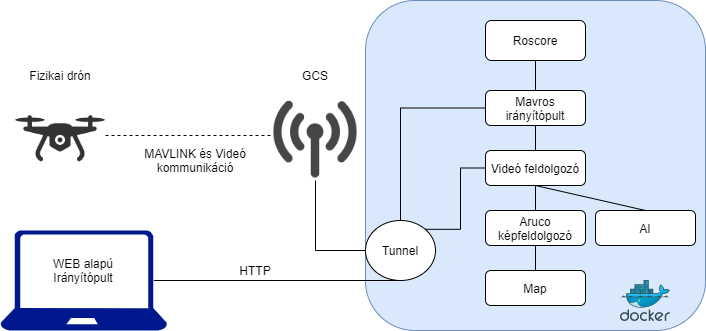
\includegraphics[width=\linewidth]{figures/vke_drone.png}
	\caption{Kész VKE földi rendszer}
	\label{fig:vke}
\end{figure}

\noindent
Ezen bemutatott rendszer az amit felhőbe integrálok, fizikai drón helyett szimulációval és leegyszerűsítve a funkciókat és a hálózati megvalósítást. A négy konténer amivel tovább dolgozom, az a Roscore, Mavros irányítópult, Aruco képfeldolgozó és ami a \ref{fig:vke}. számú ábrán nincs rajta, a PX4 alapú Gazebo szimuláció konténere. Az ábrán látható konténerek mindegyike Docker technológiával megvalósított és a \emph{drone-control-2} gyűjtőkönyvtár tartalmaz egy \emph{docker-compose.yml} fájlt, ami az adott konténerek más környezetben való összehangolásában van segítségünkre. Az egyes almappák mindegyike tartalmaz egy \emph{Dockerfile}-t, ami megmutatja, hogy Docker környezetben az adott konténer miként van létrehozva, mik a szükséges elvégzendő műveletek az alapműködésükhöz.